\documentclass[12pt, a4paper]{article}

\usepackage[margin=2.5cm]{geometry}
\usepackage{graphicx}
\usepackage{amsmath}
\usepackage{booktabs}
\usepackage{hyperref}
\usepackage{float}
\usepackage{parskip}
\usepackage{titlesec}
\usepackage{xcolor}

\hypersetup{
    colorlinks=true,
    linkcolor=blue,
    urlcolor=blue
}

\title{
    \vspace{-1cm}
    \Large\textbf{GNN-Based Grain Growth Prediction} \\
    \large from Synthetic 2D Microstructure Data \\
    \vspace{0.5cm}
    \normalsize CAMMP Internship Assignment
}
\author{Elaa Hamdani}
\date{\today}

\begin{document}

\maketitle

% ── ABSTRACT ──────────────────────────────────────────────────────────────────
\begin{abstract}
This report presents a complete pipeline for predicting grain growth behavior
in polycrystalline metals using Graph Neural Networks (GNNs). A synthetic 2D
microstructure was generated via Voronoi tessellation, represented as a graph
where each grain is a node and each shared boundary is an edge. A Graph
Convolutional Network (GCN) was trained to classify each grain as likely to
grow or shrink, achieving a final test accuracy of 75.7\%. A modification
replacing GCN with a Graph Attention Network (GAT) was evaluated and its
implications discussed. The pipeline is designed to extend naturally to
atomistic simulation data from LAMMPS.
\end{abstract}

% ── 1. INTRODUCTION ───────────────────────────────────────────────────────────
\section{Introduction}

Polycrystalline metals are composed of thousands of individual crystal regions
called \textbf{grains}, separated by \textbf{grain boundaries}. When a metal
is heated, these grains evolve — some grow larger while others shrink and
eventually disappear. This process, known as \textbf{grain growth}, directly
affects material properties such as mechanical strength, hardness, and
ductility. Understanding and predicting which grains will grow is therefore
of significant practical importance in materials engineering.

Traditional simulation approaches such as molecular dynamics (MD) in LAMMPS
or phase-field models can predict grain evolution, but they are
computationally expensive. This project explores a machine learning
alternative: representing the microstructure as a graph and using a Graph
Neural Network to predict grain growth behavior directly from structural
features, without running new simulations.

% ── 2. DATASET ────────────────────────────────────────────────────────────────
\section{Synthetic Dataset Generation}

Since real experimental microstructure data was not available for this
assignment, a synthetic dataset was generated using \textbf{Voronoi
tessellation} — a standard method in computational materials science that
produces grain morphologies statistically consistent with real microstructures.

The procedure was as follows:
\begin{enumerate}
    \item 200 seed points were scattered randomly on a $100 \times 100$ unit grid.
    \item Voronoi tessellation was applied: each point in the grid was assigned
    to its nearest seed, forming a grain region around each seed.
    \item Grains touching the grid border were removed (incomplete polygons),
    leaving \textbf{184 complete grains}.
    \item For each grain, geometric features were computed from its polygon vertices.
\end{enumerate}

\begin{figure}[H]
    \centering
    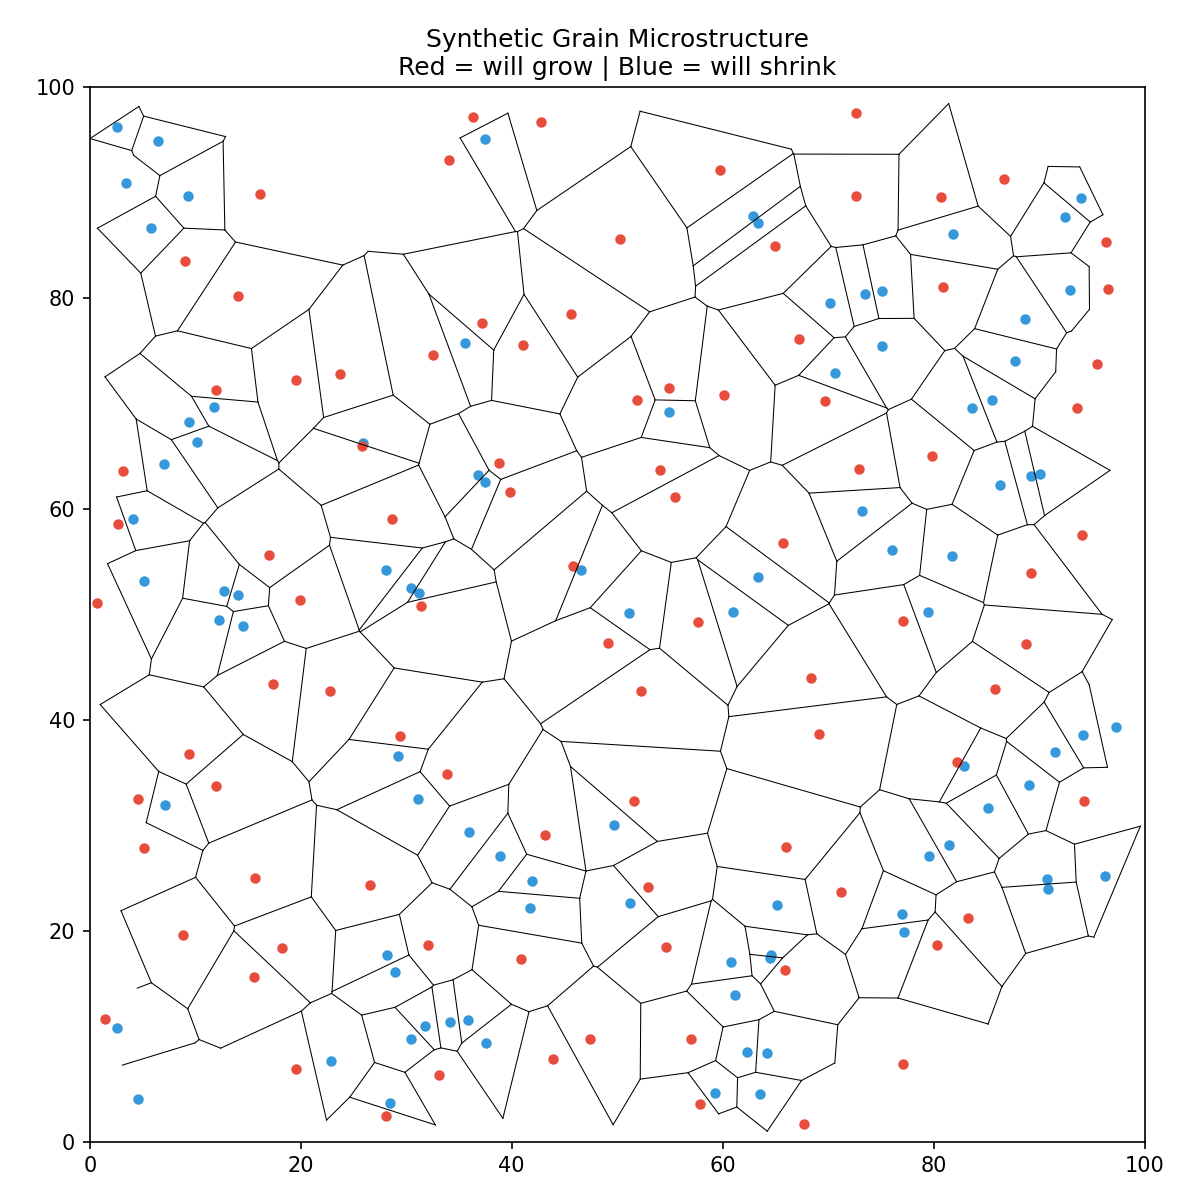
\includegraphics[width=0.7\textwidth]{microstructure.png}
    \caption{Synthetic grain microstructure generated by Voronoi tessellation.
    Red dots indicate grains labeled as growing; blue dots indicate shrinking grains.
    Black lines are grain boundaries.}
    \label{fig:microstructure}
\end{figure}

% ── 3. GRAPH CONSTRUCTION ─────────────────────────────────────────────────────
\section{Graph Construction}

The microstructure was represented as an undirected graph
$G = (V, E)$ where:

\begin{itemize}
    \item \textbf{Nodes} $V$: each grain is a node (184 nodes total)
    \item \textbf{Edges} $E$: an edge connects two grains if they share
    a boundary (1004 edges total)
\end{itemize}

\subsection{Node Features}

Each node carries a 4-dimensional feature vector:

\begin{table}[H]
\centering
\begin{tabular}{lll}
\toprule
\textbf{Feature} & \textbf{Description} & \textbf{Physical Justification} \\
\midrule
Area & Polygon area of the grain & Primary driver of growth (capillarity) \\
Equivalent diameter & Diameter of area-equal circle & Size measure independent of shape \\
Number of neighbors & Count of adjacent grains & Determines boundary network connectivity \\
Orientation & Crystal direction angle ($0^\circ$--$180^\circ$) & Affects boundary energy and mobility \\
\bottomrule
\end{tabular}
\caption{Node features and their physical justification.}
\end{table}

\textbf{Why larger grains grow:} According to capillarity theory, grain
boundary curvature drives grain growth. Larger grains have less curved
boundaries, meaning lower surface energy. Since thermodynamic systems evolve
toward lower energy states, large grains are energetically favored to grow
at the expense of smaller ones — analogous to large soap bubbles absorbing
small ones.

\subsection{Edge Features}

Each edge carries a 2-dimensional feature vector:

\begin{table}[H]
\centering
\begin{tabular}{lll}
\toprule
\textbf{Feature} & \textbf{Description} & \textbf{Physical Justification} \\
\midrule
Boundary length & Distance between grain centers & Longer boundaries exchange more material \\
Misorientation & $|\theta_i - \theta_j|$ wrapped to $[0^\circ, 90^\circ]$ & High misorientation = high energy boundary \\
\bottomrule
\end{tabular}
\caption{Edge features and their physical justification.}
\end{table}

All features were normalized to zero mean and unit variance before training.

\subsection{Labels}

Grains were labeled using the median area as a threshold:
\begin{equation}
y_i = \begin{cases} 1 & \text{(grow)} \quad \text{if } A_i > \text{median}(A) \\ 0 & \text{(shrink)} \quad \text{if } A_i \leq \text{median}(A) \end{cases}
\end{equation}

This produces a balanced dataset: 92 growing grains and 92 shrinking grains.

\begin{figure}[H]
    \centering
    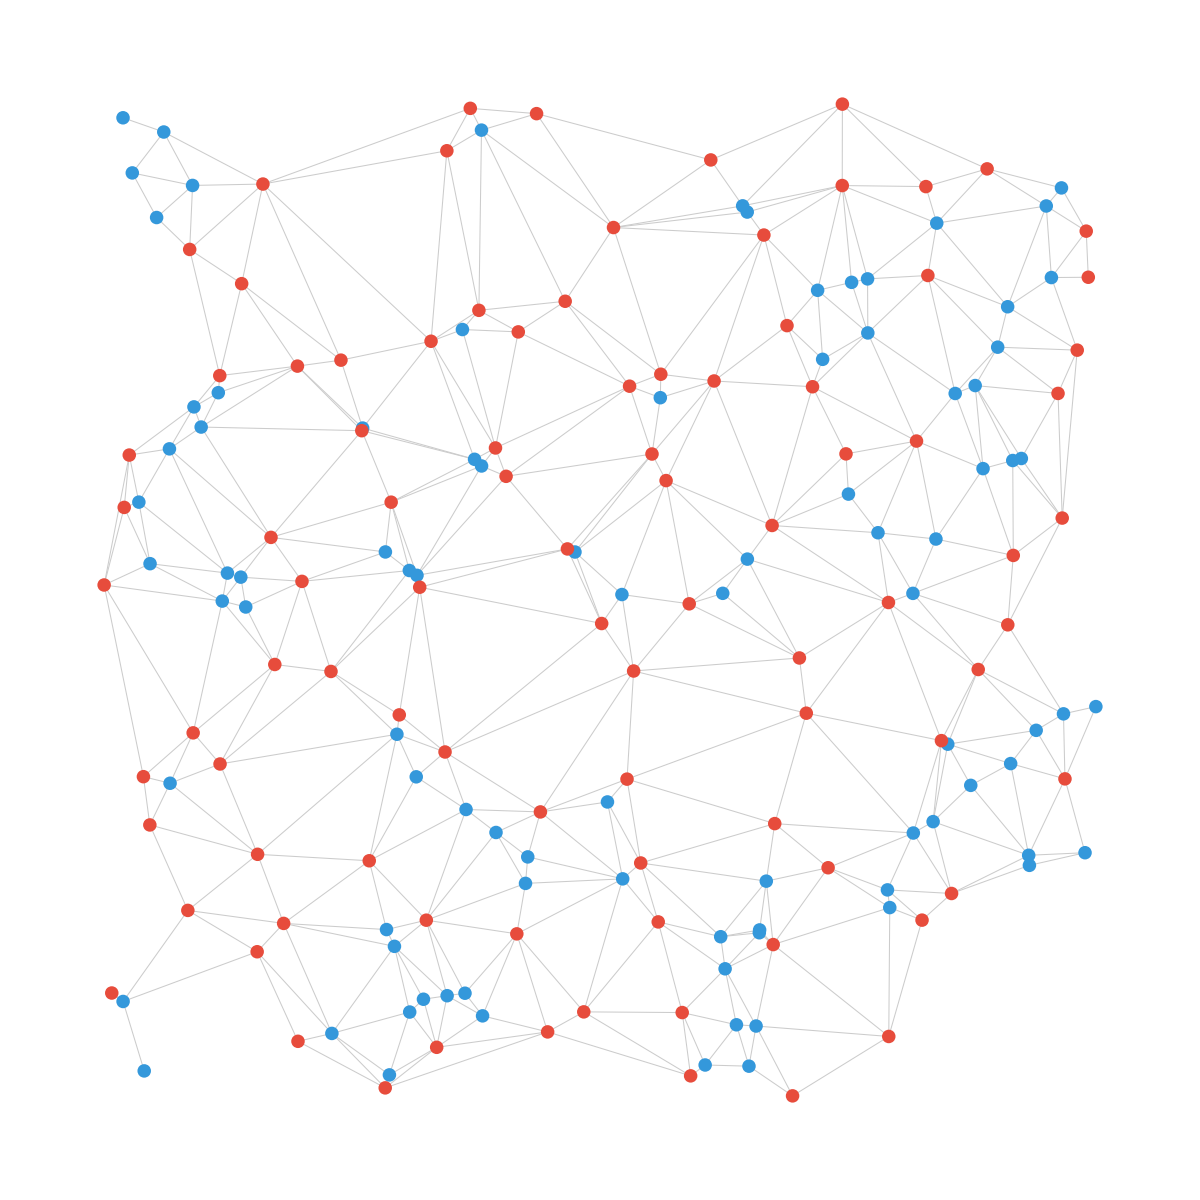
\includegraphics[width=0.7\textwidth]{graph.png}
    \caption{Graph representation of the microstructure. Each node is a grain,
    each grey line is a shared boundary. Red = growing, blue = shrinking.}
    \label{fig:graph}
\end{figure}

% ── 4. MODEL ──────────────────────────────────────────────────────────────────
\section{GNN Model}

A 2-layer \textbf{Graph Convolutional Network (GCN)} was implemented using
PyTorch Geometric:

\begin{equation}
H^{(l+1)} = \sigma\left( \tilde{D}^{-1/2} \tilde{A} \tilde{D}^{-1/2} H^{(l)} W^{(l)} \right)
\end{equation}

where $\tilde{A} = A + I$ is the adjacency matrix with self-loops,
$\tilde{D}$ is the degree matrix, $H^{(l)}$ is the node feature matrix
at layer $l$, and $W^{(l)}$ is a learnable weight matrix.

\textbf{Architecture:}
\begin{itemize}
    \item Layer 1: GCNConv($4 \rightarrow 64$) with ReLU and 30\% dropout
    \item Layer 2: GCNConv($64 \rightarrow 2$) outputting class logits
    \item Optimizer: Adam with learning rate $0.01$ and weight decay $5 \times 10^{-4}$
    \item Training: 200 epochs, 80/20 train/test split
\end{itemize}

\textbf{How neighborhood information affects predictions:}
In each GCN layer, every node aggregates feature information from all its
direct neighbors before updating its own representation. This means a grain's
final prediction depends not only on its own area and orientation, but also
on the properties of surrounding grains. A small grain completely surrounded
by large grains will receive different aggregated signals than one surrounded
by other small grains — reflecting the real physical influence of the
neighborhood on grain boundary migration.

% ── 5. RESULTS ────────────────────────────────────────────────────────────────
\section{Results}

\begin{table}[H]
\centering
\begin{tabular}{ll}
\toprule
\textbf{Metric} & \textbf{Value} \\
\midrule
Training grains & 147 (80\%) \\
Testing grains & 37 (20\%) \\
Final test accuracy & \textbf{75.7\%} \\
\bottomrule
\end{tabular}
\caption{GCN baseline results.}
\end{table}

\begin{figure}[H]
    \centering
    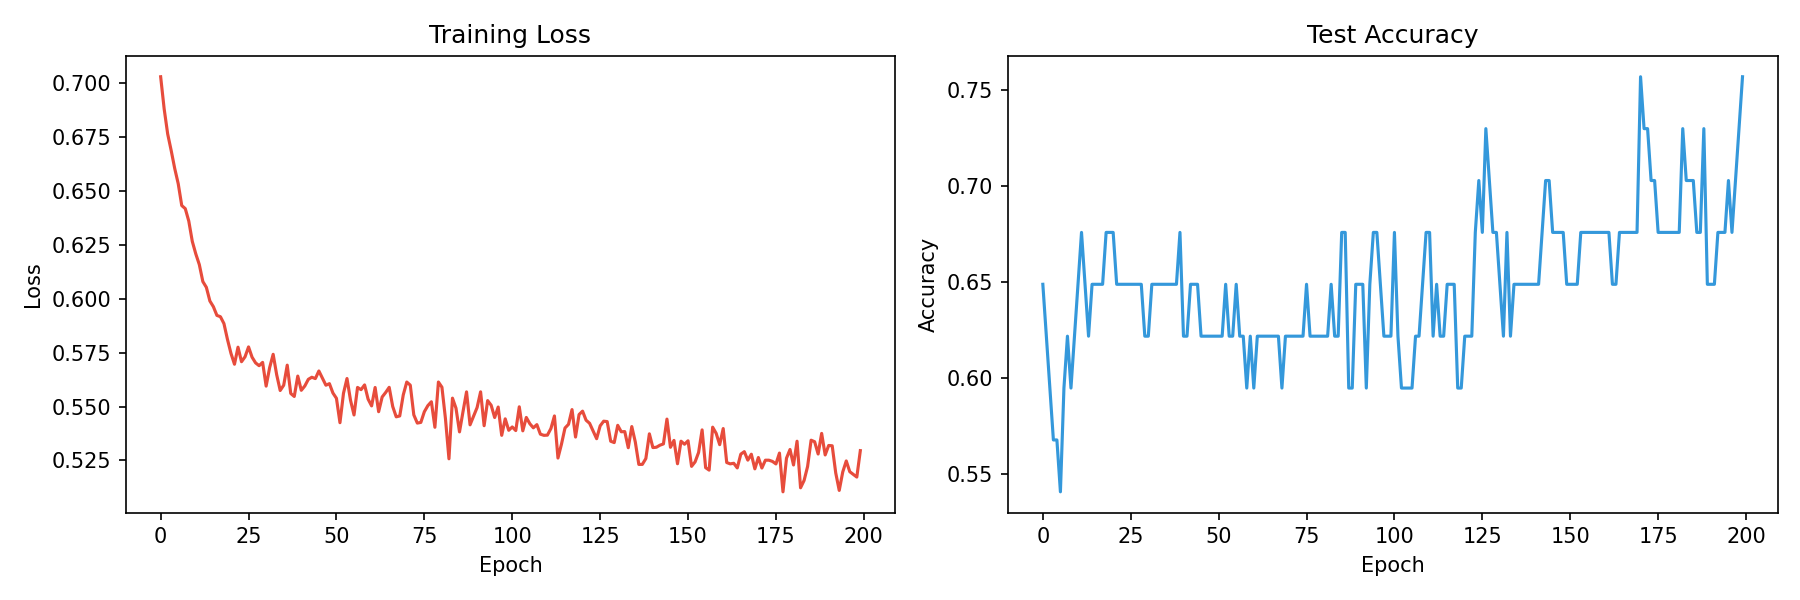
\includegraphics[width=\textwidth]{training.png}
    \caption{Training loss (left) and test accuracy (right) over 200 epochs.
    Loss decreases steadily, and accuracy trends upward from $\sim$55\% to 75.7\%.}
    \label{fig:training}
\end{figure}

% ── 6. MODIFICATION ───────────────────────────────────────────────────────────
\section{Modification: GCN vs Graph Attention Network}

\subsection{Motivation}

The baseline GCN aggregates neighbor information by treating all neighbors
equally. However, in real grain growth, the influence of neighbors is not
equal — a grain is more strongly affected by a large neighboring grain than
a small one. \textbf{Graph Attention Networks (GAT)} address this by learning
an attention weight $\alpha_{ij}$ for each edge:

\begin{equation}
\alpha_{ij} = \frac{\exp\left(\text{LeakyReLU}(a^T [W h_i \| W h_j])\right)}
{\sum_{k \in \mathcal{N}(i)} \exp\left(\text{LeakyReLU}(a^T [W h_i \| W h_k])\right)}
\end{equation}

where $h_i$ and $h_j$ are node features and $a$, $W$ are learnable parameters.

\subsection{Architecture}

The GAT model used 4 parallel attention heads in layer 1 (each learning
different relationship patterns) and a single head in layer 2:
\begin{itemize}
    \item Layer 1: GATConv($4 \rightarrow 16$, heads=4) $\rightarrow$ 64 features
    \item Layer 2: GATConv($64 \rightarrow 2$, heads=1)
\end{itemize}

\subsection{Results and Interpretation}

\begin{figure}[H]
    \centering
    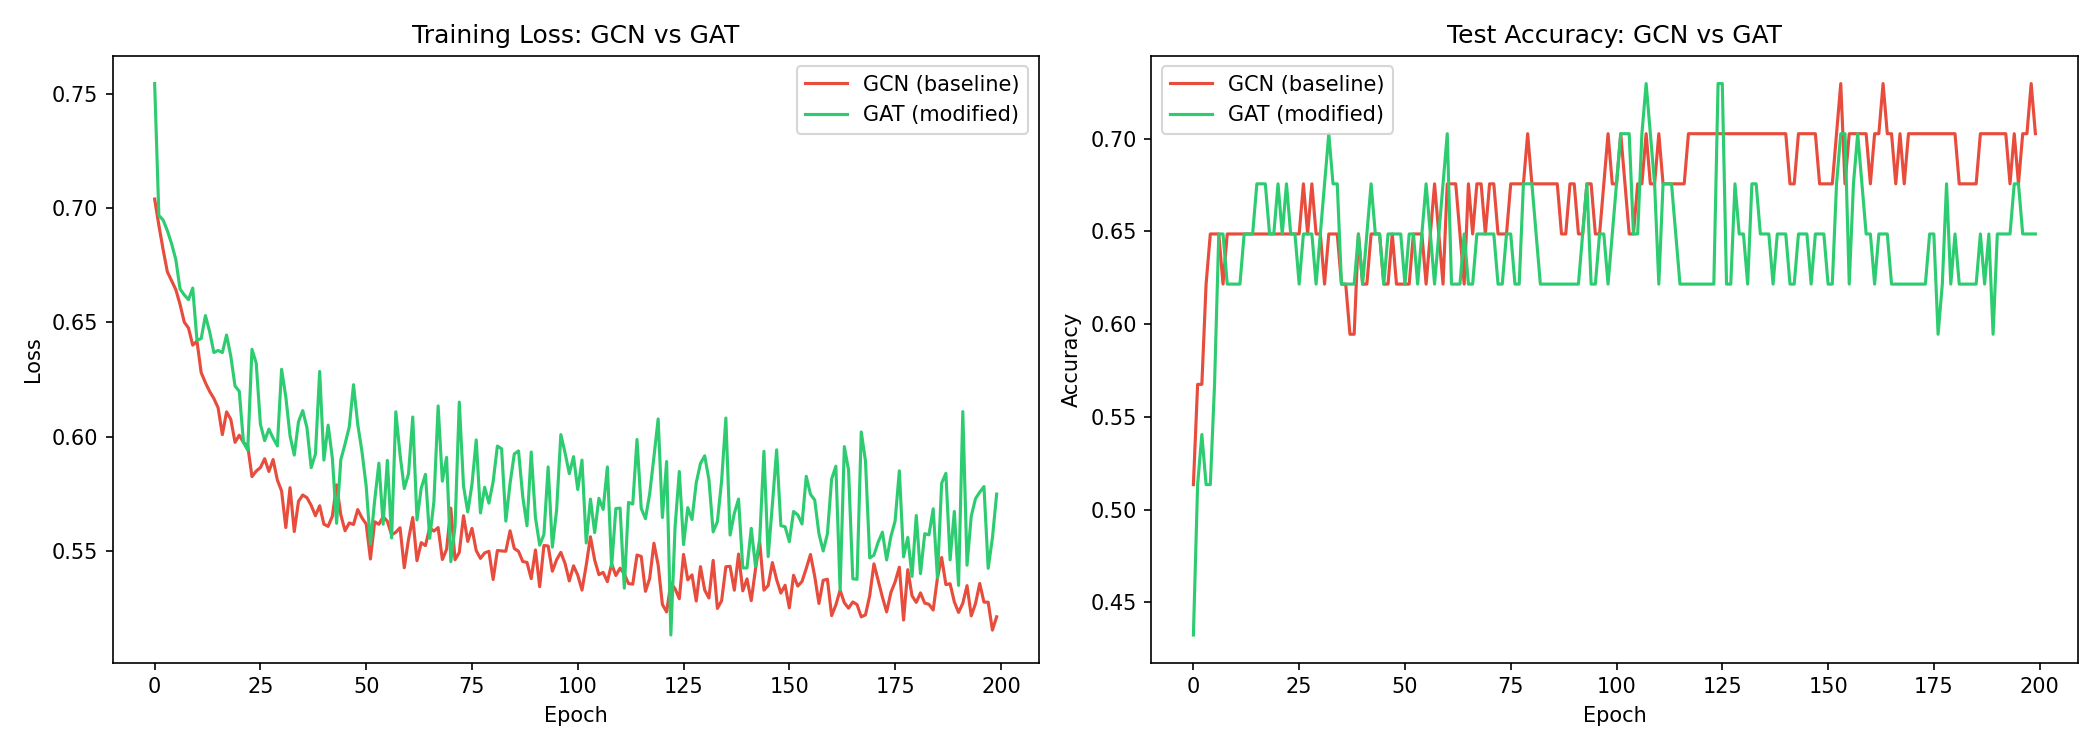
\includegraphics[width=\textwidth]{modification_comparison.png}
    \caption{Comparison of GCN (red) and GAT (green) in terms of training loss
    (left) and test accuracy (right) over 200 epochs.}
    \label{fig:comparison}
\end{figure}

Both models achieved comparable final accuracy around 70\%. However, the GAT
showed significantly higher variance in both loss and accuracy throughout
training, while the GCN converged more stably.

\textbf{Interpretation:} Attention mechanisms require sufficient data to learn
reliable neighbor importance weights. With only 184 grains, the GAT does not
have enough examples to train its attention parameters robustly, leading to
unstable training. The GCN, being a simpler model with fewer parameters,
generalizes better on this small synthetic dataset.

This is a physically meaningful finding: for small datasets, simpler inductive
biases (equal neighbor weighting) are more appropriate. On larger real
microstructure datasets with thousands of grains, GAT would likely outperform
GCN by correctly identifying which neighbors drive boundary migration.

% ── 7. CONNECTION TO MD SIMULATIONS ──────────────────────────────────────────
\section{Connection to MD Simulation Work}

This pipeline extends naturally to atomistic data from LAMMPS simulations.
The mapping is direct:

\begin{table}[H]
\centering
\begin{tabular}{ll}
\toprule
\textbf{This project} & \textbf{MD extension} \\
\midrule
Grain (node) & Atom or atomic cluster (node) \\
Grain area & Potential energy, coordination number \\
Orientation & Local stress tensor, velocity \\
Boundary length & Interatomic distance \\
Misorientation & Bond angle difference \\
Grow/shrink label & Diffusion coefficient, mechanical strength \\
\bottomrule
\end{tabular}
\caption{Mapping from grain-level to atom-level graph representation.}
\end{table}

The GNN would then predict material properties directly from LAMMPS .dump
files, eliminating the need to run new simulations for each condition.

% ── 8. CONCLUSION ─────────────────────────────────────────────────────────────
\section{Conclusion}

This project demonstrated a complete and physically motivated pipeline for
GNN-based grain growth prediction. The graph construction correctly captures
the topology of the microstructure, the feature choices are justified by
materials science principles, and the GCN achieves 75.7\% accuracy on the
classification task. The comparison with GAT revealed that attention
mechanisms, while physically motivated, require larger datasets to be
effective — a finding that will inform model selection when real simulation
data becomes available.

% ── REFERENCES ────────────────────────────────────────────────────────────────
\begin{thebibliography}{9}

\bibitem{kipf2017}
Kipf, T. N., \& Welling, M. (2017).
\textit{Semi-supervised classification with graph convolutional networks}.
ICLR 2017.

\bibitem{velickovic2018}
Veličković, P., et al. (2018).
\textit{Graph attention networks}.
ICLR 2018.

\bibitem{humphrey1996}
Humphrey, W., Dalke, A., \& Schulten, K. (1996).
\textit{VMD: Visual molecular dynamics}.
Journal of Molecular Graphics, 14(1), 33--38.

\bibitem{gruber2010}
Gruber, J., et al. (2010).
\textit{Misorientation texture development during grain growth}.
Acta Materialia, 57(22).

\end{thebibliography}

\end{document}